\section{Performance assessment}
Performance was assessed via a number of statistics. Firstly the number of lost tracks was counted. For the particle filter algorithms these were identified using the associations. When no particle was associated with the correct observation for five frames, the target was considered lost. For non-particle algorithms (PDAF and JPDAF), targets were considered lost when the mean state estimate was greater than a certain threshold distance from the correct position.

After excluding lost tracks, the RMS state error was measured. For the particle algorithms a state estimate was obtained by taking the mean of the state of all particles. For non-particle algorithms, the mean of the Gaussian representing the state distribution was used. For particle algorithms, the proportion of particles with the correct association was also calculated. These statistics were all measured at a fixed lag of five steps from the current time, for consistency of comparison.

Results are shown in table\ref{}. Blank cells indicate that the tracker failed to complete the test. With the JPDAF this occured when the number of association hypotheses grew too large.

\begin{table} \centering
\begin{tabular}{|c|c|c|c|c|c|}
\hline
 & & \multicolumn{4}{|c|}{Algorithm} \\
\hline
 & & Case 1 & Case 2 & Case 3 & Case 4 \\
\hline
\multirow{3}{*}{PDAF} & lost tracks             & 32\% & 4\% & 56\% & 50\% \\
                         & RMSE                 & 4.00 & 1.57 & 5.93 & 4.12 \\
\hline
\multirow{3}{*}{JPDAF} & lost tracks            &  & 4\% & 48\% &  \\
                         & RMSE                 &  & 1.57 & 5.89 &  \\
\hline
\multirow{3}{*}{SISR(1)} & lost tracks          & 32\% & 2\% & 100\% & 36\% \\
                         & RMSE                 & 5.53 & 1.39 &  & 7.46 \\
                         & correct associations & 72\% & 93\% &  & 63\% \\
\hline
\multirow{3}{*}{SISR(5)} & lost tracks          & 2\% & 0\% & 100\% & 16\% \\
                         & RMSE                 & 2.02 & 0.95 &  & 2.01 \\
                         & correct associations & 85\% & 93\% &  & 79\% \\
\hline
\multirow{3}{*}{RB-SISR(5)} & lost tracks       & 4\% & 0\% & FMI & 12\% \\
                         & RMSE                 & 1.95 & 1.36 & FMI & 2.90 \\
                         & correct associations & 86\% & 93\% & FMI & 83\% \\
\hline
\multirow{3}{*}{MCMC(1)} & lost tracks          & 30\% & 2\% & 100\% & 38\% \\
                         & RMSE                 & 2.24 & 1.04 &  & 1.74 \\
                         & correct associations & 87\% & 99\% &  & 81\% \\
\hline
\multirow{3}{*}{MCMC(5)} & lost tracks          & 26\% & 0\% & 100\% & 26\% \\
                         & RMSE                 & 1.44 & 0.98 &  & 1.47 \\
                         & correct associations & 87\% & 99\% &  & 81\% \\
\hline
\multirow{3}{*}{RB-MCMC(5)} & lost tracks       & 6\% & 0\% & 10\% & 12\% \\
                         & RMSE                 & 2.31 & 1.33 & 3.35 & 1.81 \\
                         & correct associations & 91\% & 99\% & 90\% & 90\% \\
\hline
\end{tabular}
\caption{Algorithm test performance measures for linear observation model}
\label{tab:ResultsLinear}
\end{table}

\begin{table} \centering
\begin{tabular}{|c|c|c|c|c|c|}
\hline
 & & \multicolumn{4}{|c|}{Algorithm} \\
\hline
 & & Case 1 & Case 2 & Case 3 & Case 4 \\
\hline
\multirow{3}{*}{PDAF} & lost tracks             & 60\% & 8\% & 80\% & 72\% \\
                         & RMSE                 & 4.89 & 2.96 & 10.15 & 5.98 \\
\hline
\multirow{3}{*}{JPDAF} & lost tracks            &  & 6\% &  &  \\
                         & RMSE                 &  & 2.95 &  &  \\
\hline
\multirow{3}{*}{SISR(1)} & lost tracks          & 40\% & 10\% & 100\% & 50\% \\
                         & RMSE                 & 9.86 & 2.54 &  & 12.93 \\
                         & correct associations & 57\% & 86\% &  & 50\% \\
\hline
\multirow{3}{*}{SISR(5)} & lost tracks          & 16\% & 4\% & FMI & 22\% \\
                         & RMSE                 & 4.51 & 1.54 & FMI & 5.91 \\
                         & correct associations & 71\% & 90\% & FMI & 69\% \\
\hline
\multirow{3}{*}{RB-SISR(5)} & lost tracks       & 18\% & 6\% & FMI & 26\% \\
                         & RMSE                 & 4.21 & 1.86 & FMI & 4.99 \\
                         & correct associations & 71\% & 89\% & FMI & 72\% \\
\hline
\multirow{3}{*}{MCMC(1)} & lost tracks          & 30\% & 2\% & 100\% & 52\% \\
                         & RMSE                 & 4.32 & 1.73 &  & 3.54 \\
                         & correct associations & 75\% & 98\% &  & 68\% \\
\hline
\multirow{3}{*}{MCMC(5)} & lost tracks          & 20\% & 4\% & 100\% & 44\% \\
                         & RMSE                 & 3.21 & 1.52 &  & 3.11 \\
                         & correct associations & 79\% & 97\% &  & 71\% \\
\hline
\multirow{3}{*}{RB-MCMC(5)} & lost tracks       & 22\% & 2\% & 48\% & 36\% \\
                         & RMSE                 & 3.36 & 1.78 & 5.96 & 3.18 \\
                         & correct associations & 80\% & 96\% & 65\% & 74\% \\
\hline
\end{tabular}
\caption{Algorithm test performance measures for bearing-range observation model}
\label{tab:ResultsRadar}
\end{table}

Figure~\ref{} to~\ref{} show the comparative performance of the algorithms on a few example cases.

\begin{figure} \centering
\subfigure[PDAF]{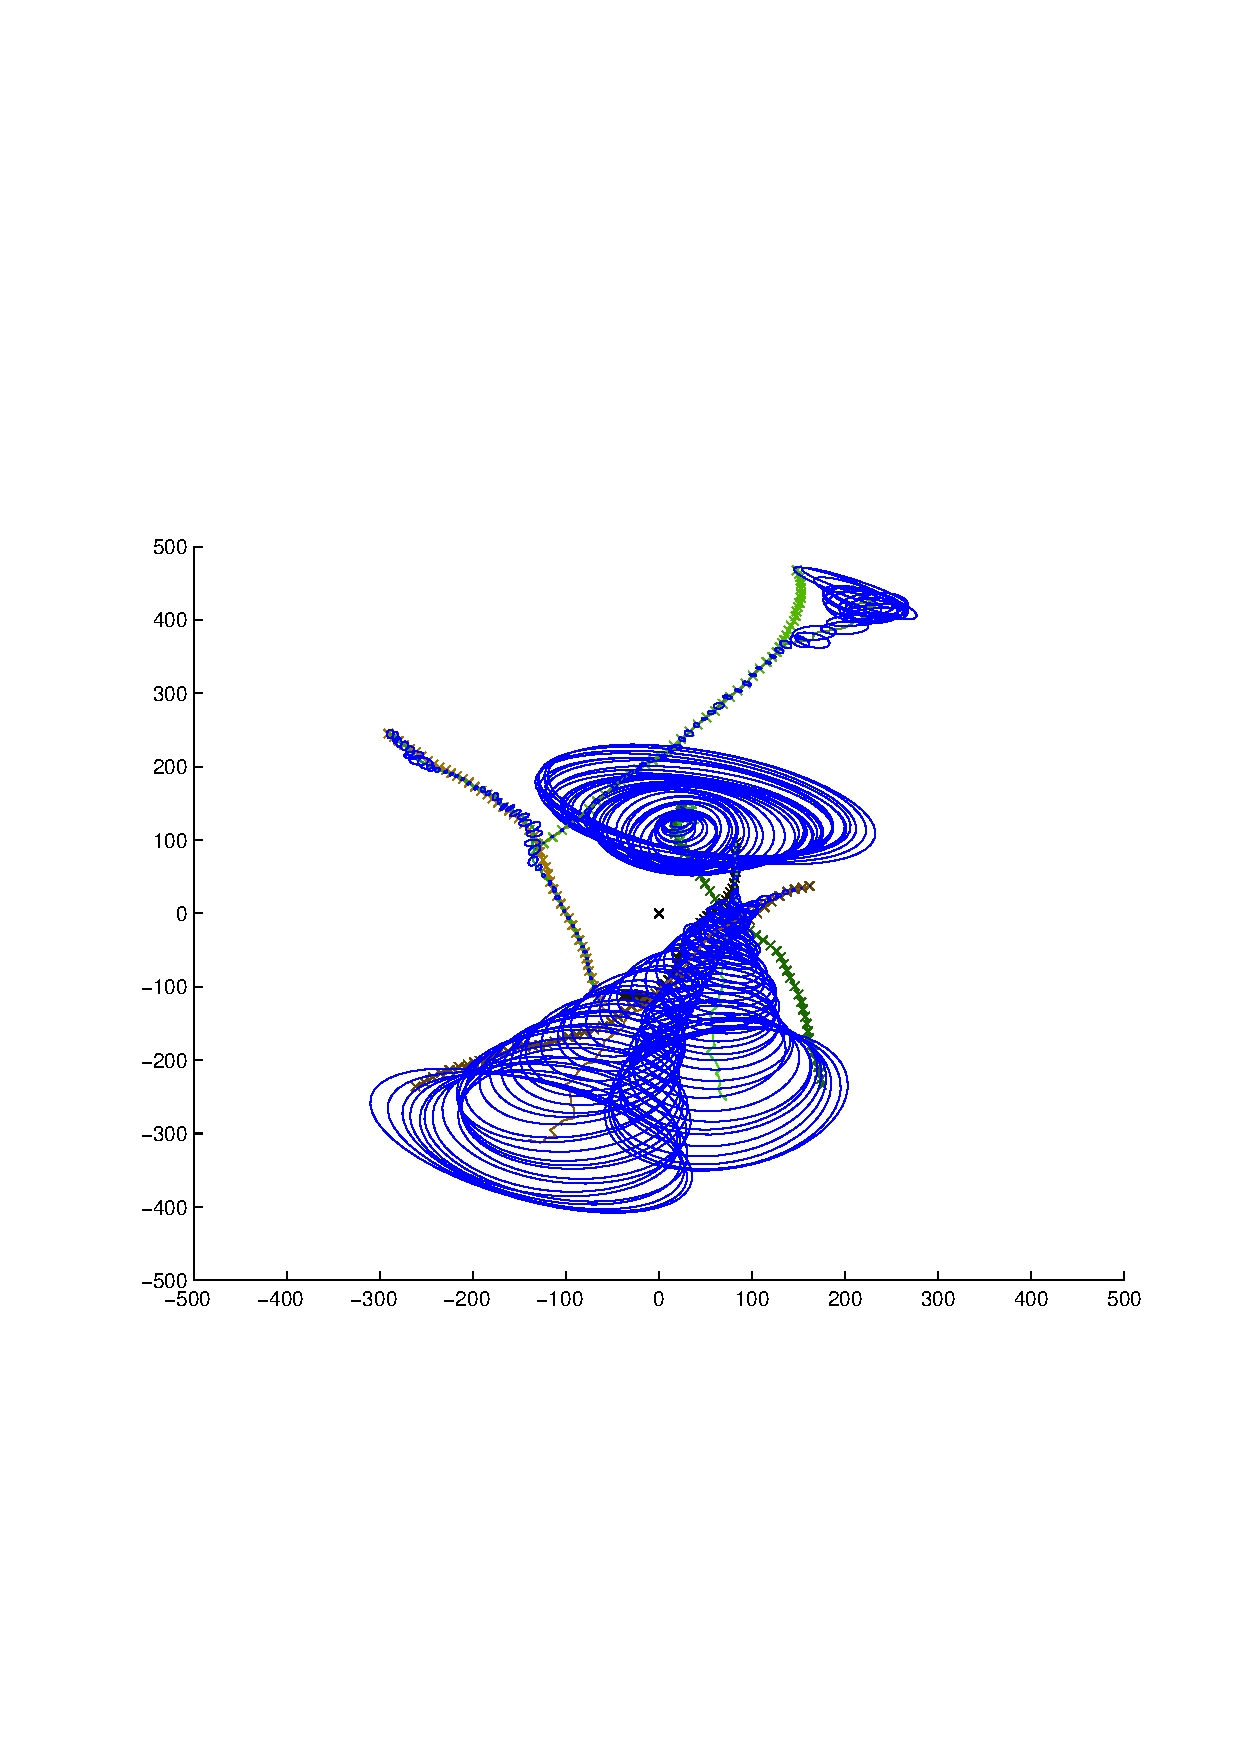
\includegraphics[width=0.49\columnwidth]{results_PDAF.pdf}}
\caption{PDAF tracking results. Ellipses mark 1 standard deviation from the mean from the Gaussian covariance estimate.}%
\label{fig:Tracking_PDAF}%
\end{figure}

\begin{figure} \centering
\subfigure[SISR(1)]{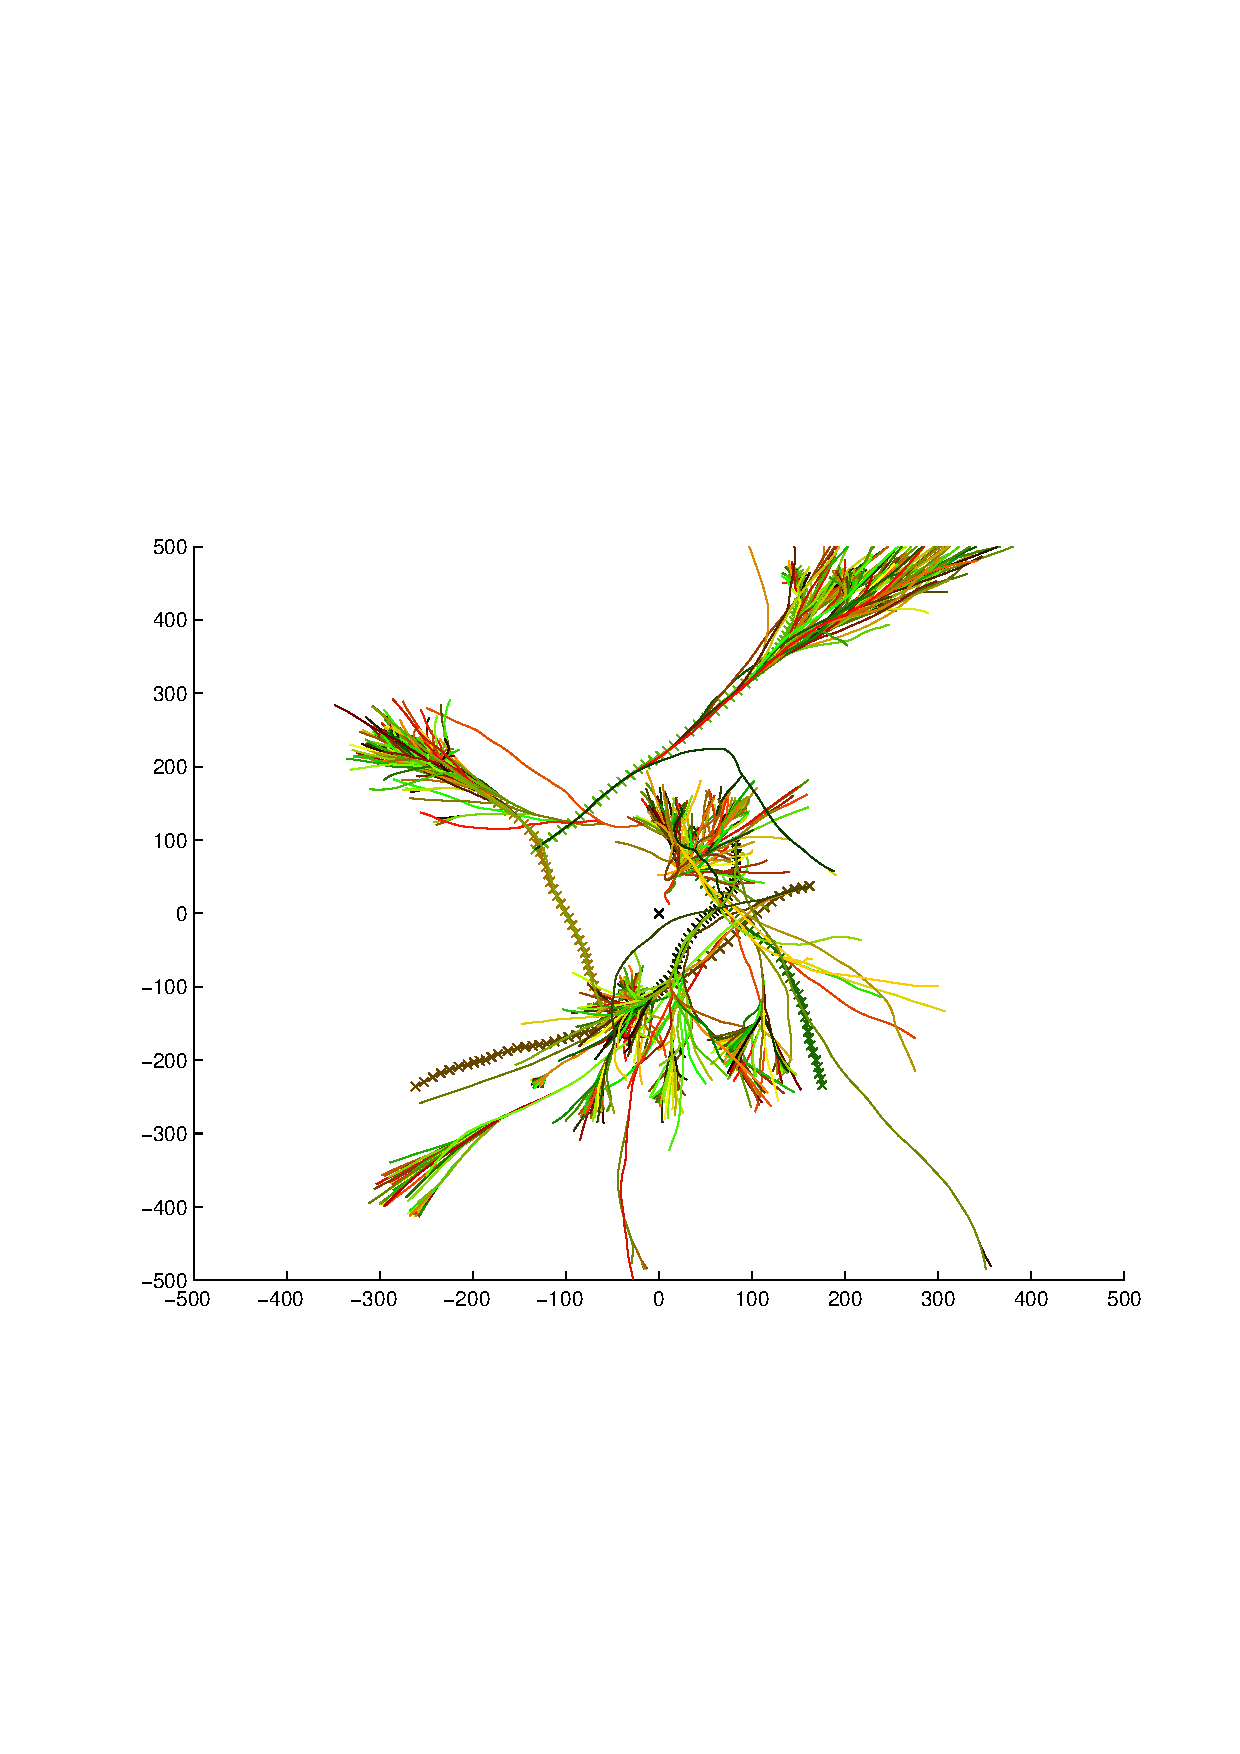
\includegraphics[width=0.49\columnwidth]{results_SISR1.pdf}}
\subfigure[SISR(5)]{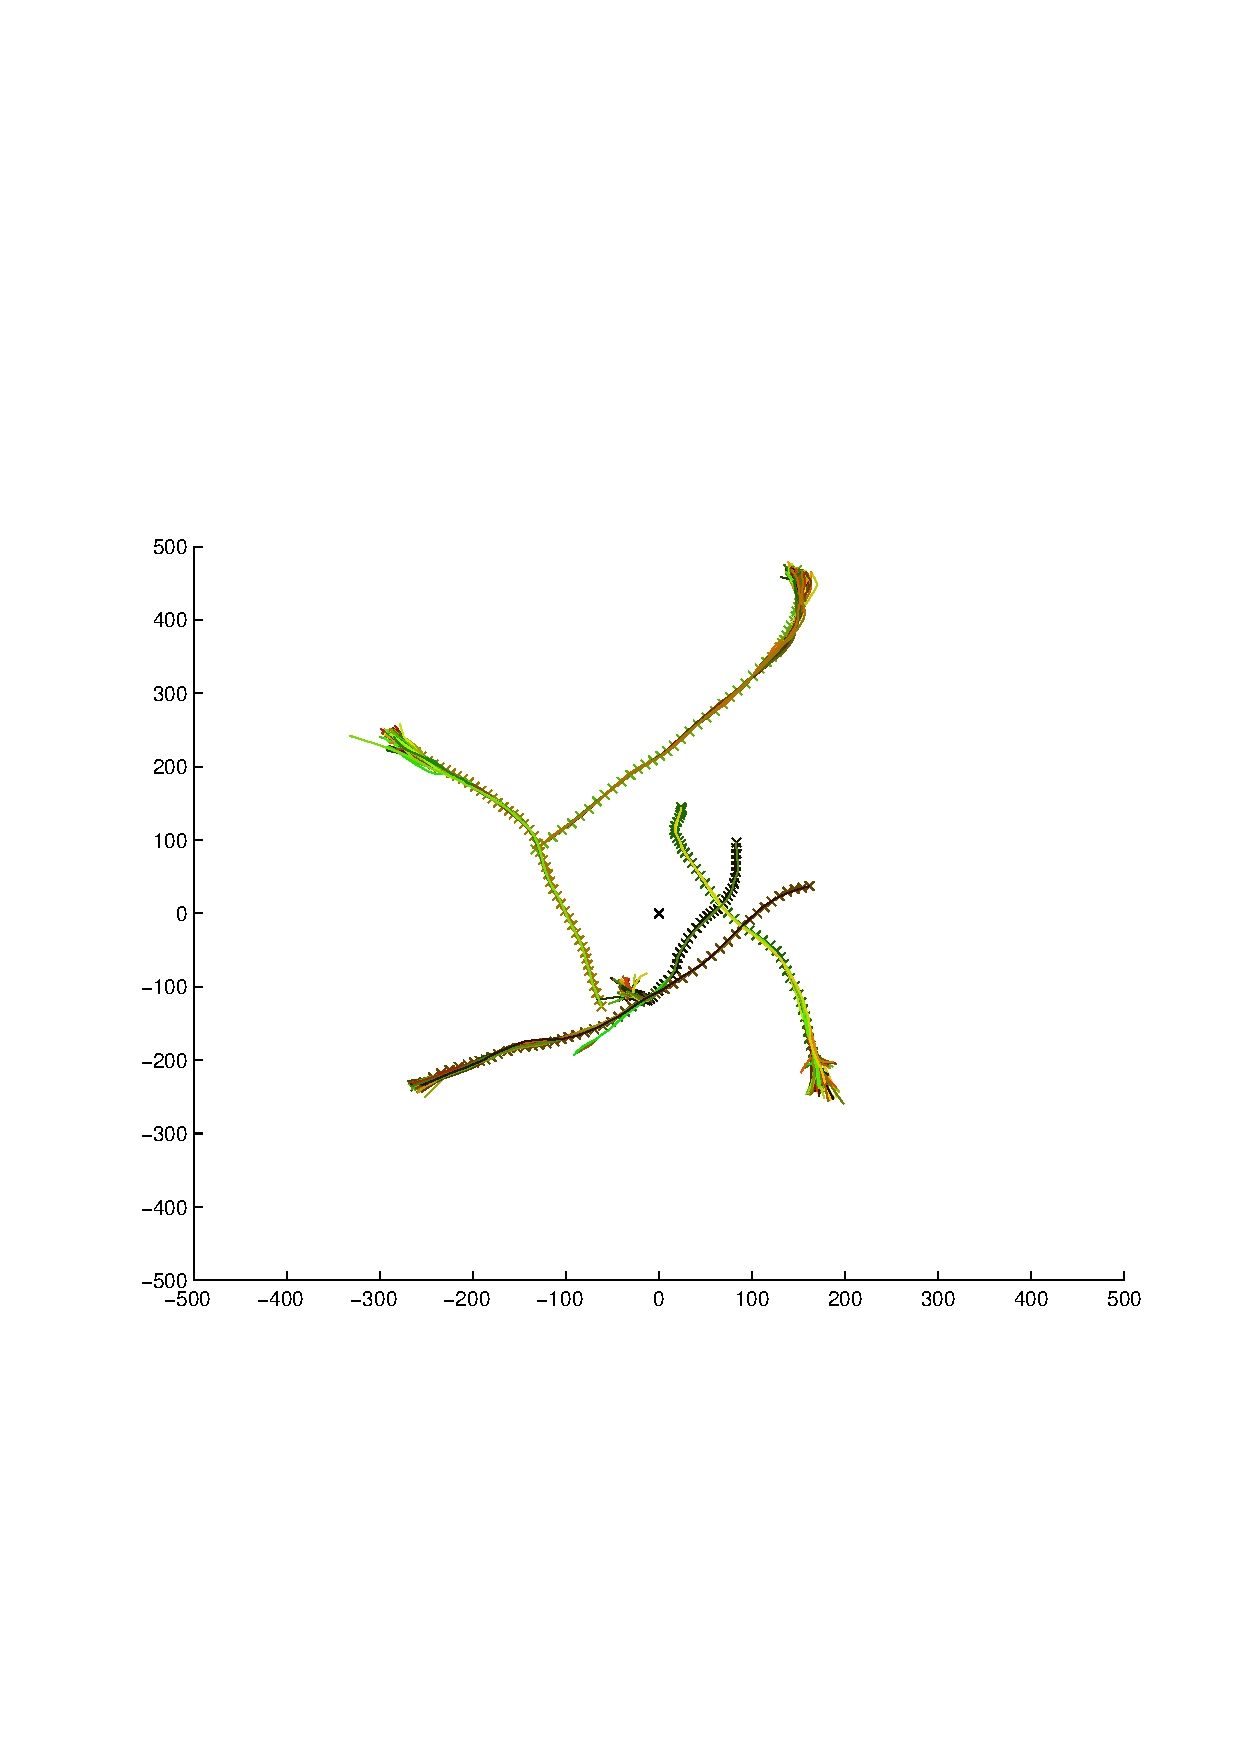
\includegraphics[width=0.49\columnwidth]{results_SISR5.pdf}} \\
\subfigure[RB-SISR(5)]{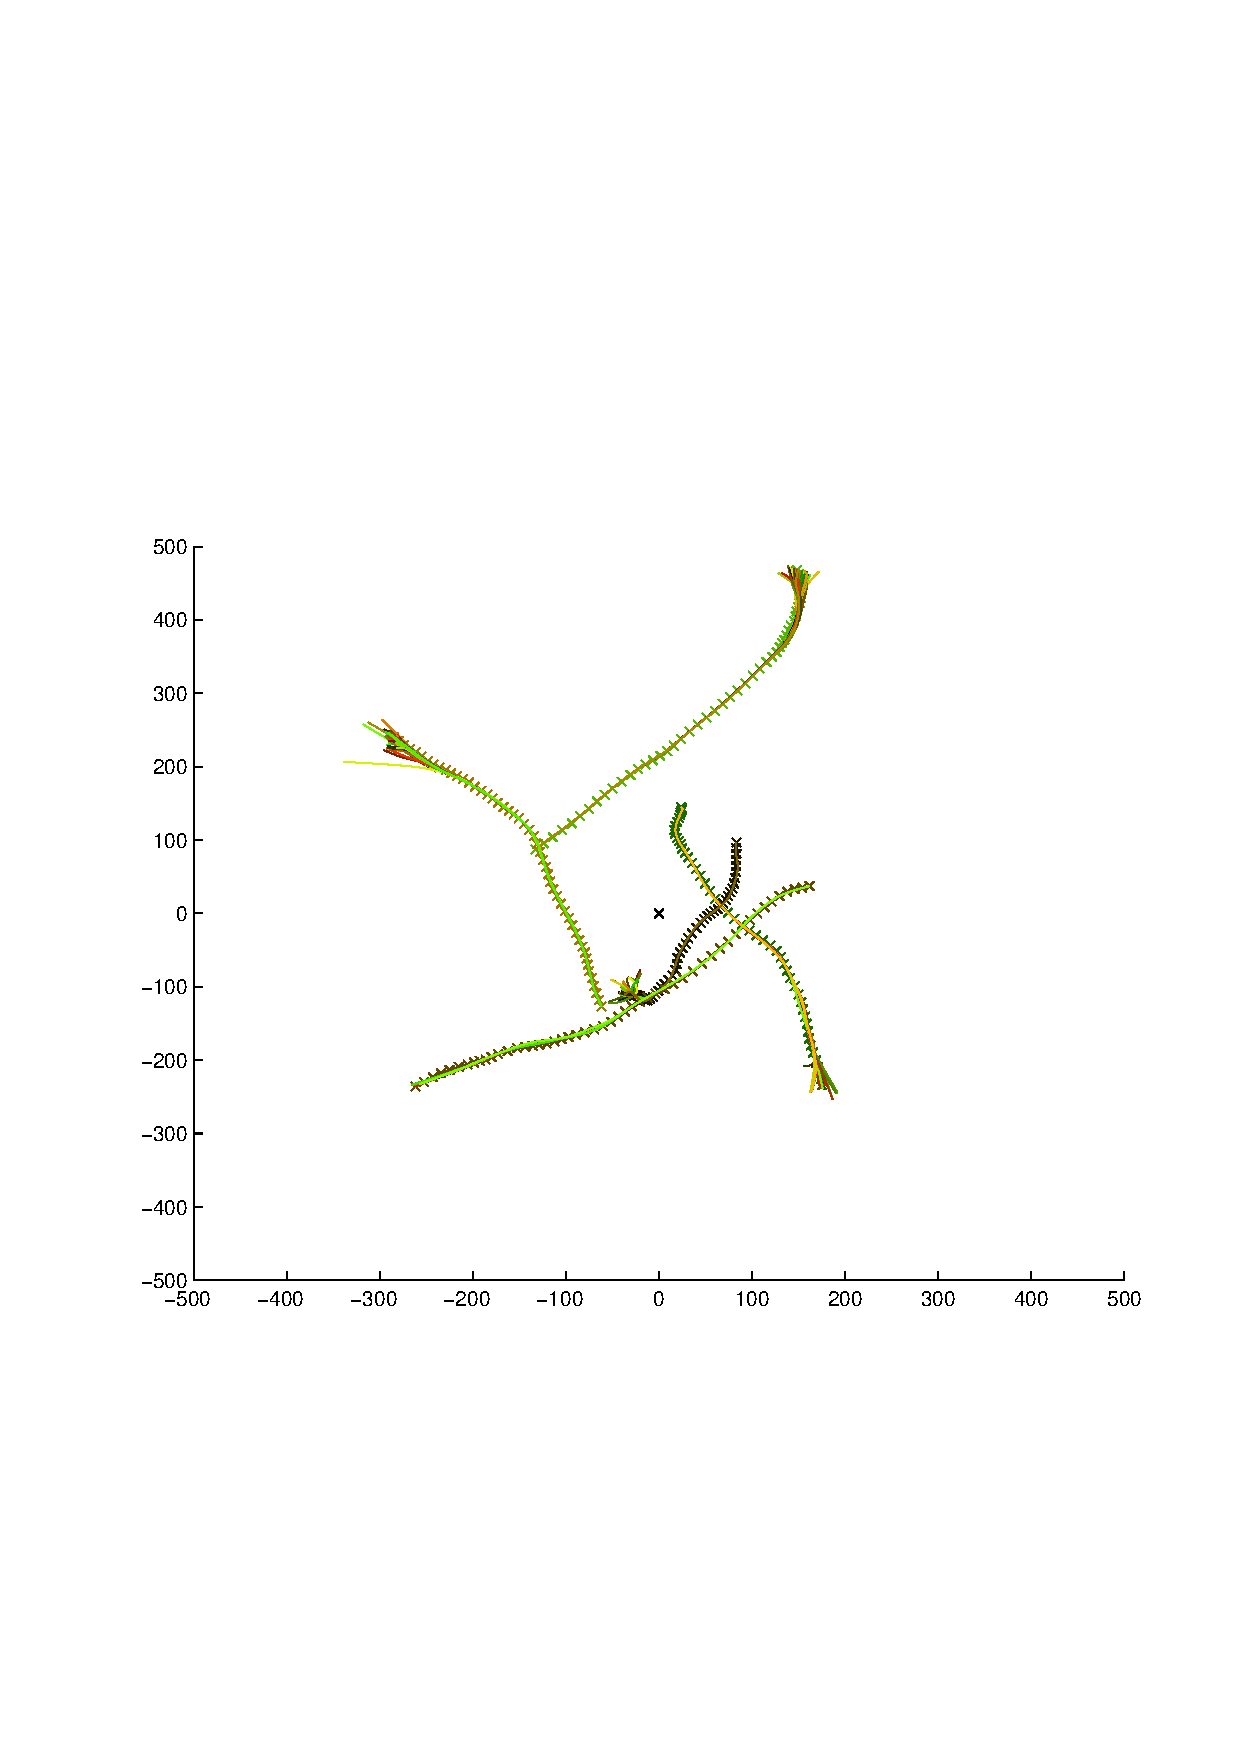
\includegraphics[width=0.49\columnwidth]{results_RB-SISR5.pdf}}
\caption{SISR tracking results. All particles plotted.}%
\label{fig:Tracking_SISR}%
\end{figure}

\begin{figure} \centering
\subfigure[MCMC(1)]{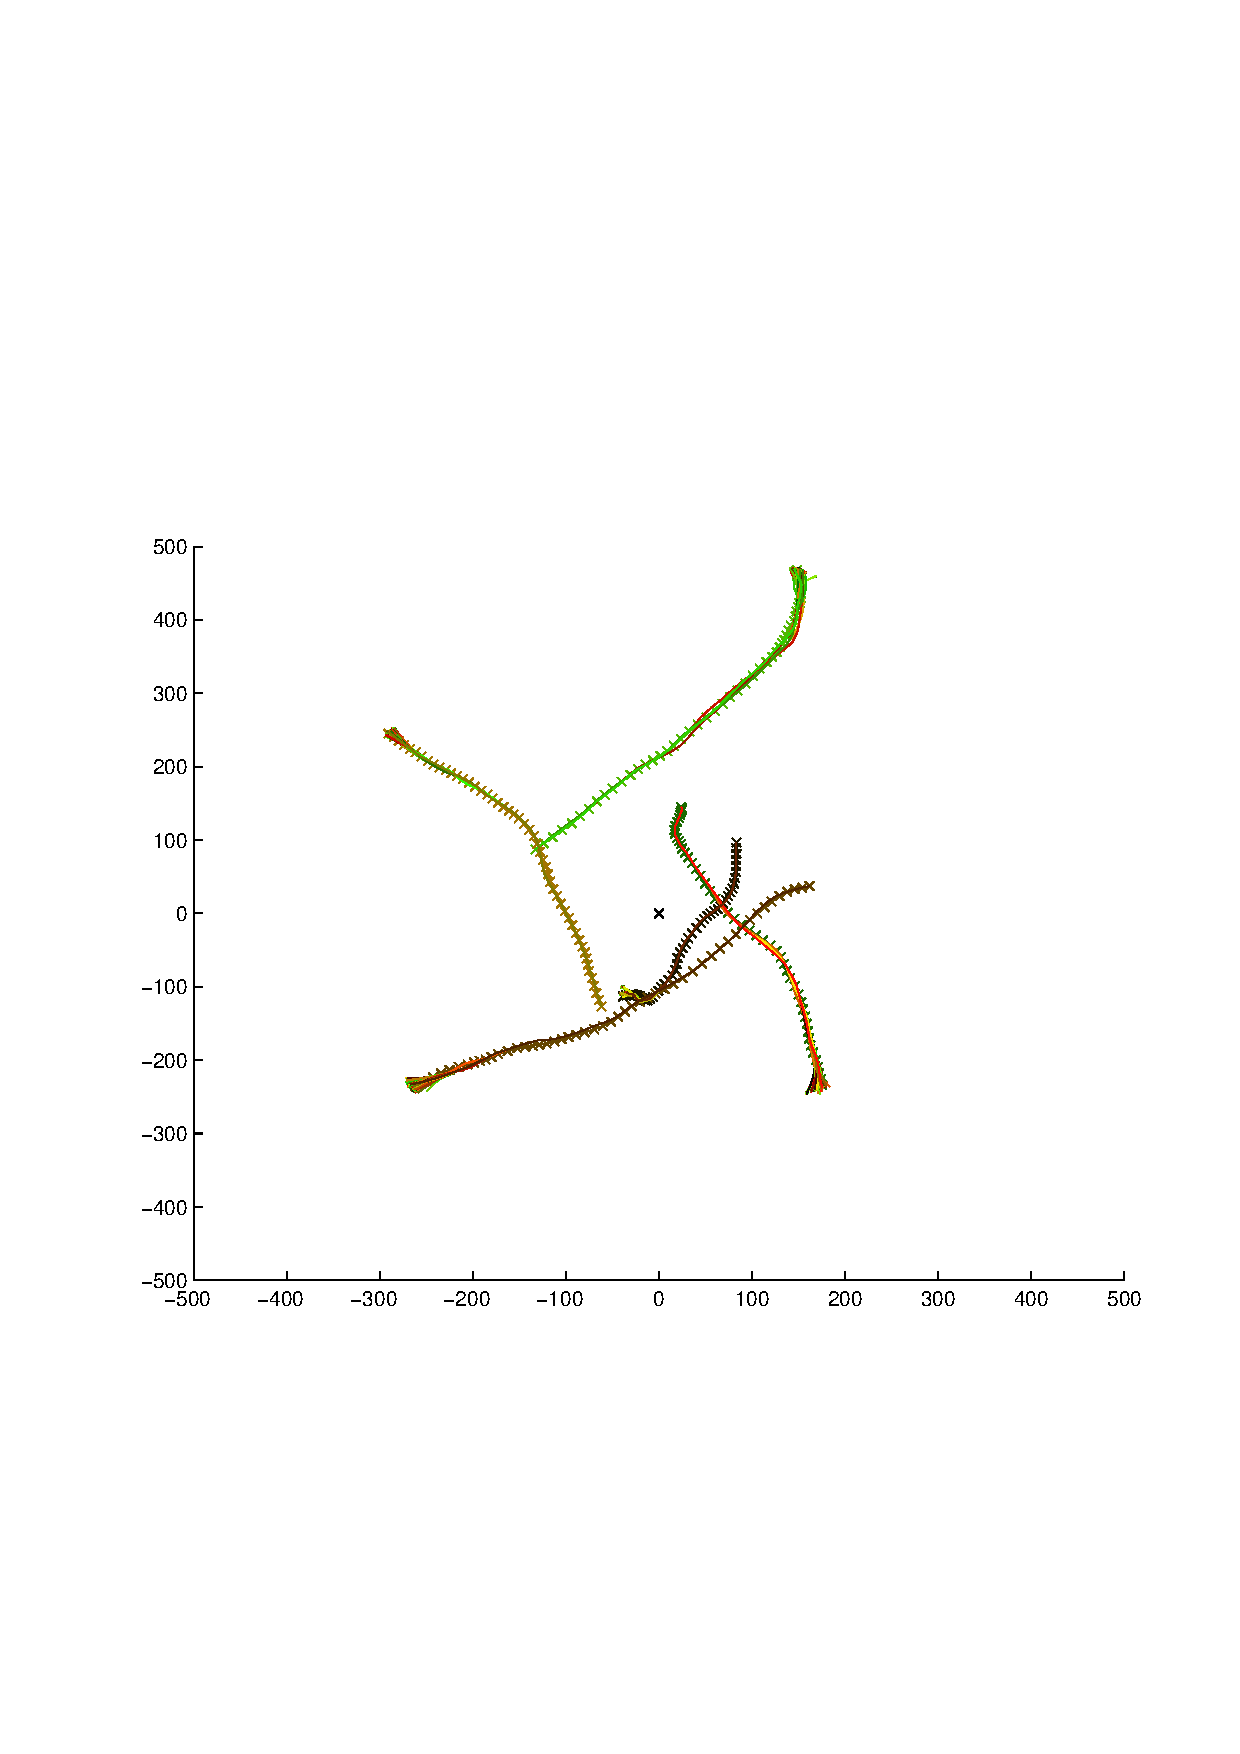
\includegraphics[width=0.49\columnwidth]{results_MCMC1.pdf}}
\subfigure[MCMC(5)]{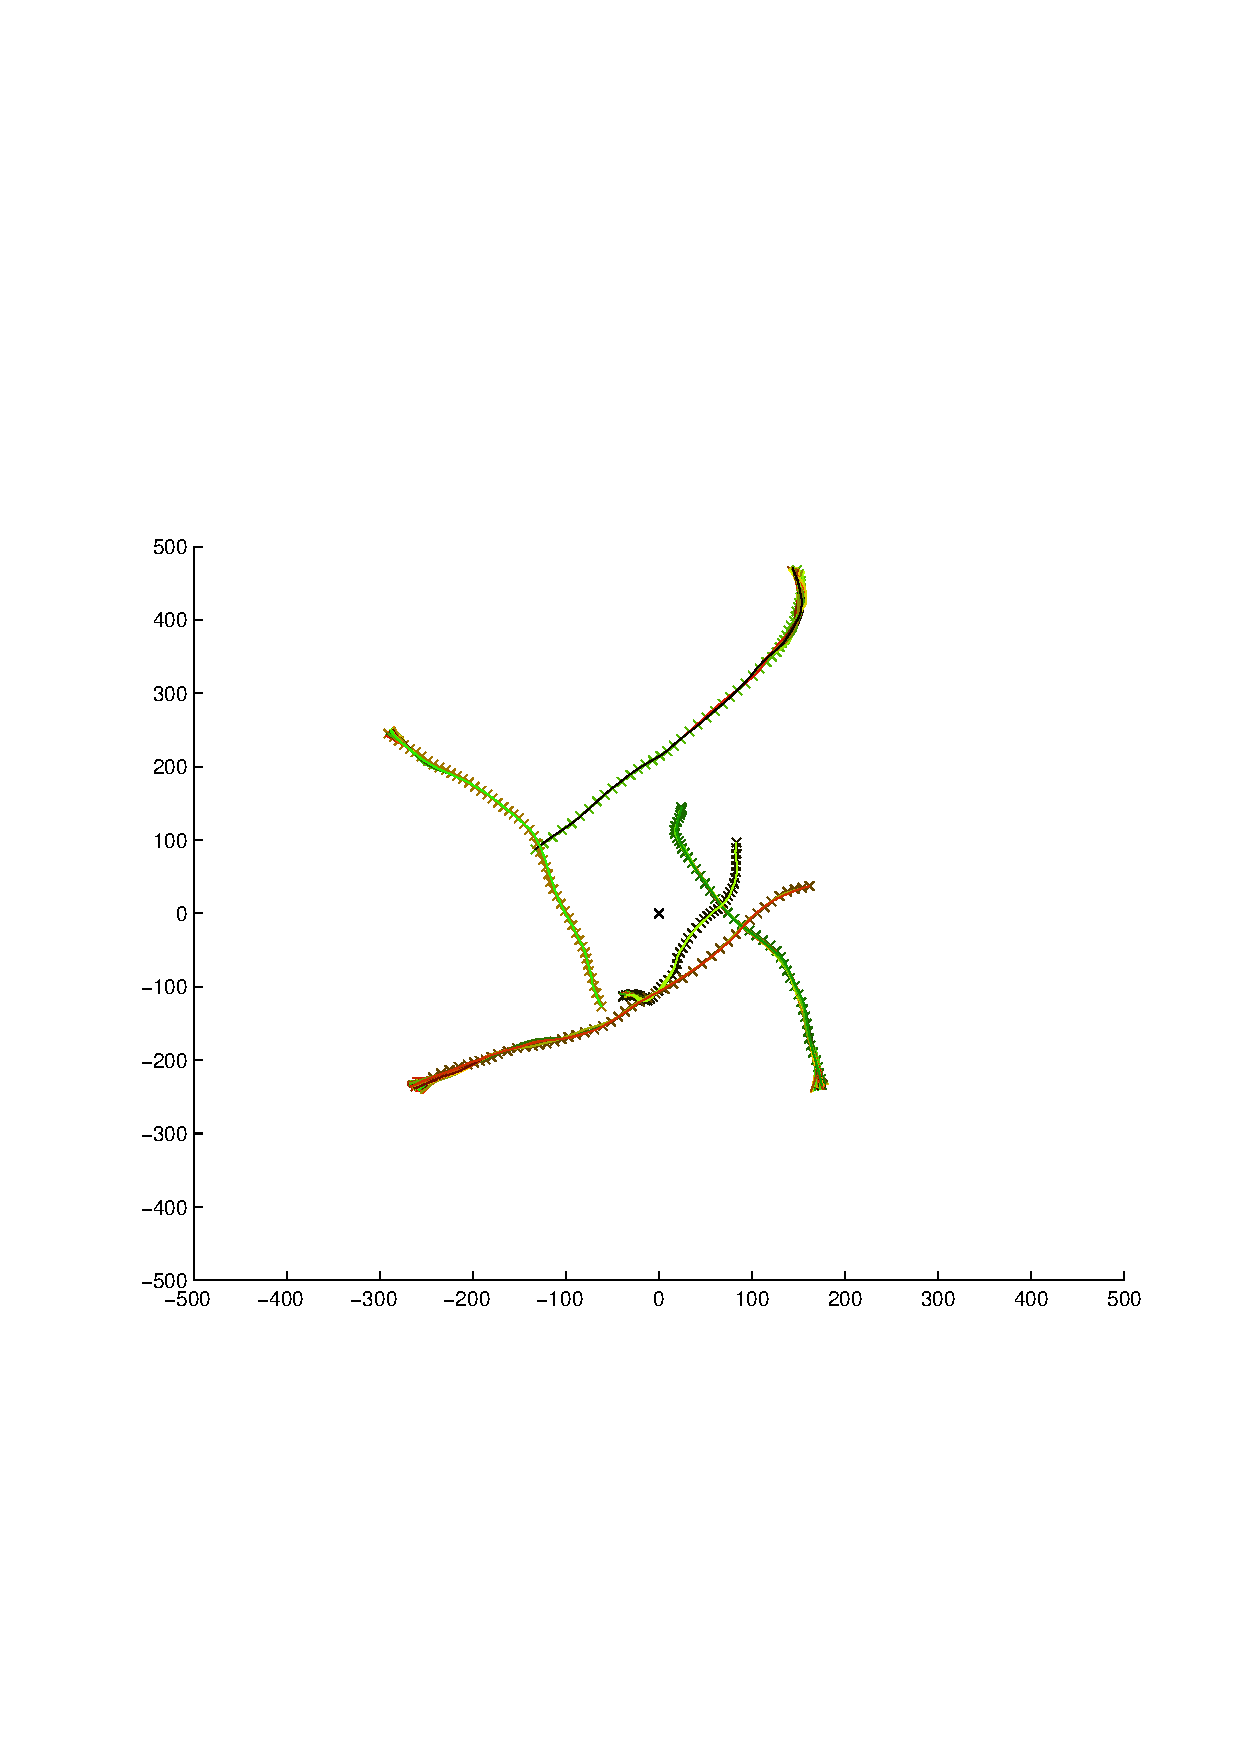
\includegraphics[width=0.49\columnwidth]{results_MCMC5.pdf}} \\
\subfigure[RB-MCMC(5)]{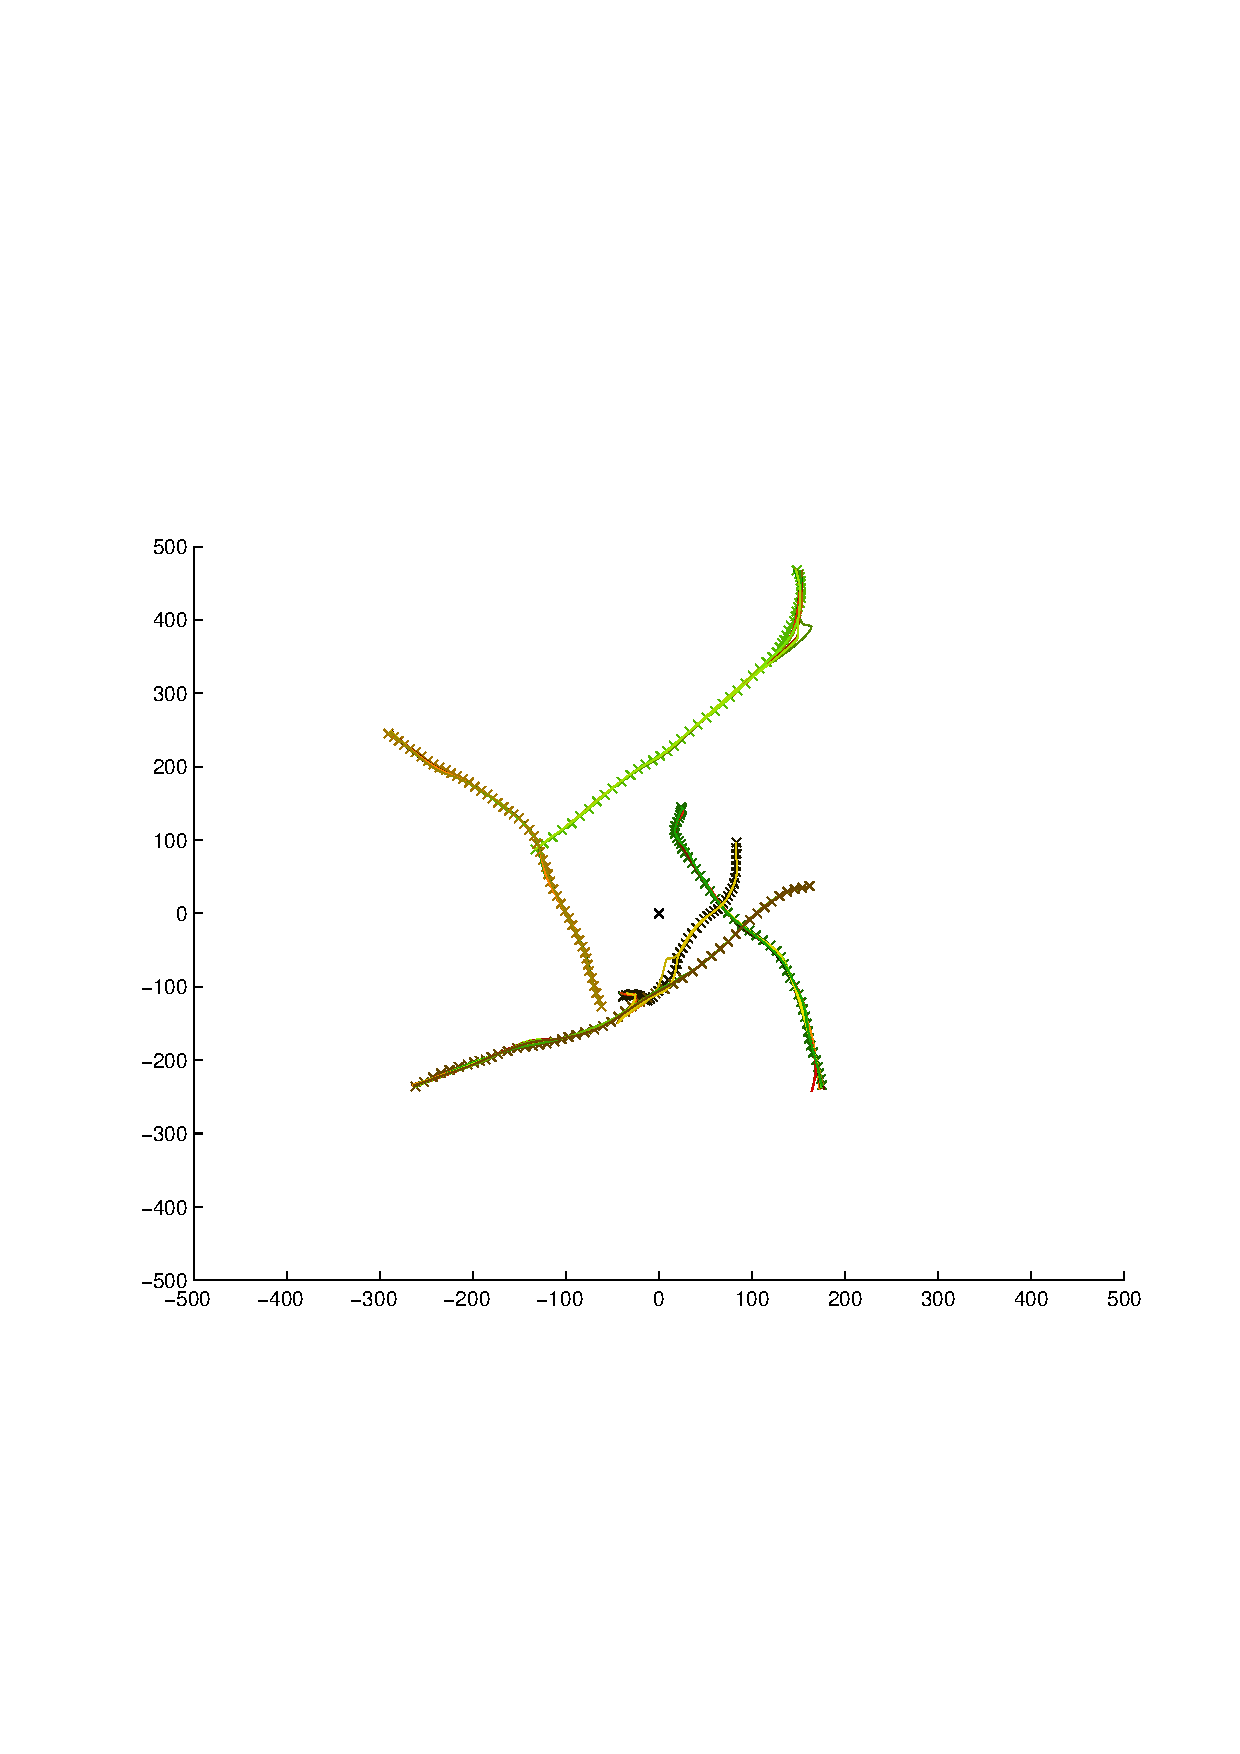
\includegraphics[width=0.49\columnwidth]{results_RB-MCMC5.pdf}}
\caption{MCMC tracking results. All particles plotted.}%
\label{fig:Tracking_MCMC}%
\end{figure}

These results highlight the characteristics of the fixed lag particle filters. In almost all cases the particle algorithms outperform the basic PDAF tracker in terms of number of tracks lost and RMSE. In all cases using a longer window results in better tracking performance. Tracking performance is always better with the linear observation model rather than the bearing-range model. For the linear model, no Gaussian approximations are needed and the proposal distributions are optimal.

For the linear observation model, the use of Rao-Blackwellisation seems to give a reduction in the number of tracks lost, and makes little difference to the RMSE. This is the expected result. The Kalman filters used for state estimation are optimal for this model, and the reduction in dimensionality means that low probability paths are better characterised, resulting in fewer track losses. With the bearing-range observation model, the reduction in lost tracks from Rao-Blackwellisation is less. This could be because the Kalman filter estimates are no longer optimal, resulting in worse state estimates and a greater tendency to follow an incorrect path. However, this hypothesis is not born out in the RMSE results, which are not significantly worse than the full particle filter.

For case 3, with high process and observation noise, the full particle filters do not work at all, while the Rao-Blackwellised forms give good tracking performance. This is because of the number of particles used is insufficient to characterise the state distribution well. The probability of getting a `good' particle becomes low, so tracks are lost very quickly. The marginalised particle filter does not need to characterise the state distribution, so the increased variance is not so significant.

On the widely spaced targets, the SISR-PFs suffer from fewer lost tracks than the MCMC-PFs. This appears to be caused by two related effects. The SISR particles are generated independently, and with the conservative resampling scheme employed a number of particles will be maintained with low weights on low probability paths. If these paths turn out to be correct, the tracker will not lose the target. The MCMC particles fail to maintain a particle contribution on such low probability paths. This may be because the particles are generated sequentially, each based upon the previous. Moves to low probability paths simply never get accepted. This problem can be viewed in an alternative light. After a few additional time steps, a low probability path which is actually correct will increase again in probability. We would like the MCMC sampler to then be able to jump across to this path. However, to do so will generally require a move in which all the states in the window (from the point at which the potential path bifurcated until the present) change significantly. Such a high dimensional move will have a very low acceptance probability, and the chains used may simply not be long enough.

Disappointingly, the MCMC-PFs do not seem to give an improvement in track loss over the SISR-PFs for the closely-spaced targets. Seeing as the MCMC-based tracker maintains a full joint distribution, it might be expected to suffer from fewer merged or crossing-over tracks. However, the difficulties outlined above seem to outweigh this potential advantage.

The particle based algorithms are of the order of 1000 times slower than the PDAF, i.e. the same order as the number of particles used. The computation time scales linearly with the length of the window. The scaling with the number of targets depends on how they interact with each other. Targets which are essentially independent (i.e. well-spaced), give rise to a linear scaling. For closely-spaced targets, the number of particles will have to increase more than linearly with the number of targets to maintain a constant level of tracking performance. The use of Rao-Blackwellisation gives the potential for a significant speed-up because many more calculations will be repeated between particles. However, this potential was not exploited in this work. The JPDAF is, while all targets remain in track, almost as fast as the PDAF. However, with a naive implementation, such as that used for these tests, the computation time explodes when a track is lost (due to the widening variance of the estimated state resulting in an increasing number of observations lying in each gate). More intelligent approaches can avoid such problems, e.g. \cite{Horridge2006}.